\documentclass[12pt]{article}
\usepackage[utf8]{inputenc}
\usepackage[english]{babel}
%\usepackage[latin1]{inputenc}
%\usepackage[norsk]{babel}
\usepackage[T1]{fontenc,url}
\usepackage{xcolor}
\usepackage{color}

\usepackage[parfill]{parskip} % Begin paragraphs with an empty line rather than an indent

%%Document formating
\usepackage[margin=1.0in]{geometry} %Set document margin (2.54cm)

%%Sections layout
\usepackage{sectsty}
\sectionfont{\fontsize{12}{15}\selectfont}
\subsectionfont{\fontsize{10}{15}\selectfont}
\sectionfont{\centering \color{purple}} %centering and color
\subsectionfont{\color{purple}}  % sets color of subsections
\renewcommand \thesection{\arabic{section}.}
\renewcommand{\thesubsection}{\thesection\arabic{subsection}}

%%Figure & tables
\usepackage{graphicx}
\usepackage{subfig}
\usepackage{float}
\usepackage{caption} % Figure & table caption
\captionsetup{labelfont={normal, bf}, font={it}}

%% Math environment
\usepackage{amsmath}
\usepackage{amssymb}
\usepackage{mathtools}
\usepackage{braket}
\usepackage{bm} %Bold char. in math env. Usage: $A\bm{x}=\bm{b}$
\numberwithin{equation}{section}     % Eq. numbering
%\numberwithin{equation}{subsection} % Eq. numbering

\usepackage[framemethod=TikZ]{mdframed}
\mdfsetup{skipabove=4pt,skipbelow=1pt}
\mdfdefinestyle{MyFrame}{%
    linecolor=black,
    outerlinewidth=1pt,
    roundcorner=10pt,
    innertopmargin=\baselineskip,
    innerbottommargin=\baselineskip,
    innerrightmargin=10pt,
    innerleftmargin=10pt,
    backgroundcolor=gray!10!white}
% mdframed usage:
%\begin{mdframed}[style=MyFrame]
% $E = mC^2$
%\end{mdframed}

%% Referencing
\urlstyle{sf}
\usepackage{hyperref} %Auto create hyperlinks within the document
\hypersetup{          %Set color of referenced items to 'blue'
    colorlinks=true,
    linkcolor=blue,
    filecolor=blue,
    urlcolor=blue,}

%% Code formating
\usepackage{listings}
\definecolor{codegreen}{rgb}{0,0.6,0}
\definecolor{codegray}{rgb}{0.5,0.5,0.5}
\definecolor{codepurple}{rgb}{0.58,0,0.82}
\definecolor{backcolour}{rgb}{0.95,0.95,0.92}
\lstdefinestyle{mystyle}{
    backgroundcolor=\color{backcolour},
    commentstyle=\color{codegreen},
    keywordstyle=\color{blue},
    numberstyle=\tiny\color{codegray},
    stringstyle=\color{codepurple},
    basicstyle=\small,
    breakatwhitespace=false,
    breaklines=true,
    captionpos=b,
    keepspaces=true,
    numbers=none,
    numbersep=5pt,
    showspaces=false,
    showstringspaces=false,
    showtabs=false,
    tabsize=2
}
\lstset{style=mystyle}

%% Self-defined
\newcommand{\BigO}[1]{\ensuremath{\operatorname{O}\bigl(#1\bigr)}}

%% Begin document
\begin{document}
\title{Project 1\\FYS3150/4150}
\author{Lasse Braseth, Nicolai Haug, and Kristian Wold}
\date{September 10, 2018}
\maketitle

\begin{abstract}
It went OK. Results can be found further down.

In this project the solution of the one-dimensional Poisson equation, a second-order differential equation, is approximated numerically with three different algorithms based on recasting the Poisson equation as a tridiagonal matrix equation. The first algorithm .. second algorithm .. third algorithm .. Testing the algorithms on a case with a known closed form, it was found that all algorithms approximated the solution satisfactory for a relatively low number of grid points. Comparing the CPU times of each algorithm, it was found that ..
\end{abstract}

\pagenumbering{gobble}
\thispagestyle{empty}
\newpage
\pagenumbering{arabic}

\section{Introduction}
This project explores three different numerical algorithms for solving the Poisson equation, a second-order differential equation, recast as a tridiagonal matrix by discretization. The first algorithm, labeled “General Algorithm”, use the Gaussian elimination procedure and backward substitution. The second algorithm, labeled “Optimized Algorithm”, is an optimalization of the General Algorithm by specializing it to the specific matrix spawned by the discretization of the Poisson equation, known as a Toeplitz matrix. The third algorithm, labeled “LU-decomposition Algorithm” use the built-in LU-decomposition method in the C++ library Armadillo. The subject of particular interest in this project is the computational performance of the algorithms. This will be studied by comparing the difference in FLOPS (floating point operations per second) and computational time between the algorithms. A study of the numerical error produced by the approximations and machine error will also be carried out, as well as a visual comparison between a known closed form of the Poisson equation and the numerical solution.

This project is structured by first presenting an theoretical overview of the problem, followed by a derivation of the aforementioned algorithms. Next, the results from the implementation of the algorithms are presented, before lastly they and the approach are discussed and concluded upon.



In this project we study how to discretize and recast Poisson's equation as a tridiagonal matrix equation. We explore different methods of how to solve these sets of equations. First we develop an algorithm for solving a general tridiagonal matrix using Gaussian elimination and backwards substitution. Next we optimize the algorithm by specializing it to the specific matrix spawned by the discretization of the equation, known as a Toeplitz matrix. We also check the difference in FLOP's and computational time between the different methods. Next we study the numerical error produced by discretization and machine error using the optimized method and compare this to expected error caused by our way of discretizing. Lastly, we
solve the matrix equation yet again using LU-decomposition imported from the Armadillo library. We compare the results with our previous methon and investigate the limitations of Armadillo with respect to computational time and memory usage.

To solve this equation numerically we have to discretize it, and we will then show how this discretization will give rise to a matrix equation. We are so to solve this equation using two different methods, the first method is the Gaussian elimination procedure, and for tridiagonal matrices also known as the Thomas algorithm. The second method is the LU decomposition method. In the first part of the project we will give a theoretical overview of the problem, and in the second part we will give a derivation of the different algorithms we will implement. In the third part we will represent the results, before we lastly discuss our approach and the results we found.

\section{Theory}
\subsection{The Poisson Equation}
The Poisson equation is a classical equation from electromagnetism that describe the electrostatic potential generated by a localized charge distribution. In electromagnetism it assumes the following form

\begin{equation}\label{Poisson}
     \nabla^{2}\phi(\vec{r})=-4\pi\rho(\vec{r})
\end{equation}
By assuming that both $\phi$ and $\rho$ are spherically symmetric, the equation is just dependent on the distance from the source
\begin{align}
    \nabla_{r}^{2}\phi(r)=-4\pi\rho(r),
\end{align}
where the gradient squared is given by
\begin{align}
    \nabla_{r}^{2}=\frac{1}{r^{2}}\frac{d}{dr}\left(r^{2}\frac{d}{dr} \right)
\end{align}
Which gives us that the equation take the form
\begin{align}
    \frac{d^{2}\phi(r)}{dr^{2}}=-4\pi r\rho(r)
\end{align}
As we see the equation is now a one dimensional problem, so let us do the substitutions $\phi\rightarrow u$ and $r\rightarrow x$. Then the equation can be represented in the following way
\begin{equation}\label{u''}
    -u''(x)=f(x)
\end{equation}
Where we have the conditions $x\in(0,1)$ and the boundary conditions $u(0)=u(1)=0$. In this project we study the source term
\begin{equation}\label{source}
    f(x) = 100e^{-10x}
\end{equation}
with the known closed form solution
\begin{equation}\label{solution}
    u(x) = 1 - (1 - e^{-10})x - e^{-10x}
\end{equation}

\subsection{Approximation to the Second Derivative}
In order to solve this equation numerically we have to discretize it. Let us start of by doing a Taylor expansion for u(x)
\begin{align*}
    u(x\pm h)=u(x)\pm hu'+\frac{h^{2}}{2}u''\pm \frac{h^{3}}{3!}u'''+\BigO{h^{4}}
\end{align*}
Now we take the sum of the two
\begin{align*}
    u(x+h)+u(x-h)=2u(x)+h^{2}u''+\BigO{h^{4}}
\end{align*}
If we solve this equation for $u''$ we have the approximation for the second derivative
\begin{align*}
    u''=\frac{u(x+h)+u(x-h)-2u(x)}{h^{2}}+\BigO{h^{2}}
\end{align*}
Now if we connect this to \eqref{u''} we see that our differential equation has the discrete form
\begin{equation}
    -\frac{v_{i+1}+v_{i-1}-2v_{i}}{h^{2}}=f_{i}
\end{equation}
The boundary conditions are $v_{0}=v_{n+1}=0.$ If we now write out the explicit terms we get
\begin{align*}
    -v_{2}+2v_{1}&=h^{2}f_{1}\\
    -v_{3}-v_{1}+2v_{2}&=h^{2}f_{2}\\
    -v_{4}-v_{2}+2v_{3}&=h^{2}f_{3}\\
    \vdots\\
    -v_{n}-v_{n-2}+2v_{n-1}&=h^{2}f_{n-1}\\
    -v_{n-1}+2v_{n}&=h^{2}f_{n}
\end{align*}
And we immediately see that this is exactly the same as writing\\\\
\begin{align*}
\begin{bmatrix}
2& -1& 0 &\dots   & \dots &0 \\
-1 & 2 & -1 &0 &\dots &\dots \\
0&-1 &2 & -1 & 0 & \vdots \\
 & \dots   & \dots &\dots   &\dots & \dots \\
 0&\dots   &  &-1 &2& -1 \\
0&\dots    &  & 0  &-1 & 2 \
\end{bmatrix}
\begin{bmatrix}
  v_{1}  \\
  v_{2}  \\
  v_{3}  \\
  \vdots \\
  v_{n-1} \\
  v_{n}
\end{bmatrix}
= h^{2} \begin{bmatrix}
  f_{1}  \\
  f_{2}  \\
  f_{3}  \\
  \vdots \\
  f_{n-1} \\
  f_{n}
\end{bmatrix},\\
\end{align*}

Thus we obtain the matrix equation
\begin{align*}
    A\bm{v}=\bm{\tilde{f}}
\end{align*}

\subsection{Analytical error}
The function $u(x)$ is approximated with a Taylor expansion
\begin{align*}
    u(x\pm h)=u(x)\pm hu'+\frac{h^{2}}{2}u''\pm \frac{h^{3}}{3!}u'''+\BigO{h^{4}}
\end{align*}
The approxiamtion for the second derivative was found to be
\begin{equation*}
    u''=\frac{u(x+h)+u(x-h)-2u(x)}{h^{2}}+\BigO{h^{2}}
\end{equation*}
An important aspect when truncating an expansion is to find the error. When approximating to second order the error is of order $h^{2}$. The omitted terms in the expansion can be written as
\begin{equation}\label{eq:aerror}
    2\sum_{j=1}^{\infty}\frac{f(x)^{(2j+2)}}{(2j+1)!}h^{2j}
\end{equation}
So by setting $j=1$ in \eqref{eq:aerror} the approximated error is given by
\begin{equation}
    \epsilon_{approx}=\frac{f^{(4)}}{12}h^{2}
\end{equation}
So the error can be made small by setting h as small as possible. But in a computer this is not possible, so we need an extra term due to loss of numerical precision. So the total error can be written as
\begin{equation*}
    \epsilon=\epsilon_{approx}+\epsilon_{M}
\end{equation*}




\section{Method}
\subsection{Gaussian Elimination with a General Tridiagonal Matrix}

We will solve the set of linear equations $\mathbf{Av=f}$ by first applying a forward substitution followed by a backward substitution. The matrix $A$ is called a tridiagonal matrix and we can thus define three vectors $\boldsymbol{a}$, $\boldsymbol{b}$ and $\boldsymbol{c}$ which contains all the diagonal terms. In order to show the flow of the algorithm we use a $4x4$ matrix
\begin{align*}
    \begin{pmatrix}
 b_1&  c_1&  0& 0\\
 a_1&  b_2&  c_2& 0\\
 0&  a_2&  b_3& c_3\\
 0&  0&  a_3& b_4
\end{pmatrix}
\begin{pmatrix}
v_1\\
v_2\\
v_3\\
v_4
\end{pmatrix}
=
\begin{pmatrix}
f_1\\
f_2\\
f_3\\
f_4
\end{pmatrix}
\end{align*}
We want to eliminate the lower diagonal to make the matrix upper-diagonal. To knock out $a_1$, we can multiply the first row by $a_1/b_1$ and subtract it from the second
\begin{align*}
    \begin{pmatrix}
 b_1&  c_1&  0& 0\\
 0&  b_2-\frac{a_1}{b_1}c_1&  c_2& 0\\
 0&  a_2&  b_3& c_3\\
 0&  0&  a_3& b_4
\end{pmatrix}
\begin{pmatrix}
x_1\\
x_2\\
x_3\\
x_4
\end{pmatrix}
=
\begin{pmatrix}
f_1\\
f_2-\frac{a_1}{b_1}f_1\\
f_3\\
f_4
\end{pmatrix}
\end{align*}
To eliminate further, we treat $b_2-\frac{a_1}{b_1}c_1$ as the new value for $b_2$ and we treat $f_{2}-\frac{a_{1}}{b_{1}f_{1}}$ as the new value for $f_{2}$. If we now carry out the same method for the next rows we eventually have a upper diagonal matrix of the form
\begin{align*}
    \begin{pmatrix}
 b^{*}_1&  c_1&  0& 0\\
 0&  b^{*}_2&  c_2& 0\\
 0&  0&  b^{*}_3& c_3\\
 0&  0&  0& b^{*}_4
\end{pmatrix}
\begin{pmatrix}
v_1\\
v_2\\
v_3\\
v_4
\end{pmatrix}
=
\begin{pmatrix}
f^{*}_1\\
f^{*}_2\\
f^{*}_3\\
f^{*}_4
\end{pmatrix}
\end{align*}
Where we have the following equations
\begin{align*}
    b^{*}_{1}&=b_{1}\\
    b^{*}_{i}&=b_{i}-\frac{a_{i-1}c_{i-1}}{b_{i-1}^{*}}\\
    f^{*}_{1}&=f_{1}\\
    f^{*}_{i}&=f_{i}-\frac{a_{i-1}f_{i-1}^{*}}{b_{i-1}^{*}}
\end{align*}
We implement these equations in the following algorithm
\begin{lstlisting}[language=c++]
for(int i=1; i<n; i++)
{
    temp = a[i]/b[i]
    b[i+1] = b[i+1] - temp*c[i]
    f[i+1] = f[i+1] - temp*f[i]
}
\end{lstlisting}

Note that we update $b$ and $f$ in the loop, so we do not need to make new vectors $b^{*}$ and $f^{*}$. The $c$ diagonal stays the same during the elimination, since the elements above is always zero. We need not carry out the calculations for changing the a-values either, since they will be zero after the elimination. Now all the diagonal terms are pivot elements, so the forward substitution is done.

To perform a backward substitution, we look at the upper diagonal matrix and multiply the last line with $c_3/b_3$ and subtract that from the third line which results in
\begin{align*}
    \begin{pmatrix}
 b^{*}_1&  c_1&  0& 0\\
 0&  b^{*}_2&  c_2& 0\\
 0&  0&  1& 0\\
 0&  0&  0& b^{*}_4
\end{pmatrix}
\begin{pmatrix}
v_1\\
v_2\\
v_3\\
v_4
\end{pmatrix}
=
\begin{pmatrix}
f^{*}_1\\
f^{*}_2\\
f^{*}_3-\frac{c_3f^{*}_4}{b^{*}_4}\\
f^{*}_4
\end{pmatrix}
\end{align*}
We further eliminate $c_2$ by defining $f^{*}_3-\frac{c_3f^{*}_4}{b^{*}_{4}}$ as the new value for $v_3$ and do the same procedure as above. This results in the following equation
\begin{align*}
    v_{i}&=(f^{*}_i-v_{i+1}c_i)/b^{*}_i
\end{align*}
$v_i$ is implemented in the following algorithm
\begin{lstlisting}[language=c++]
for(int i=n-2; i>0; i--)
{
    v[i] = (f[i]-c[i]*v[i+1])/b[i]
}
\end{lstlisting}
A important aspect in numerical computations is the efficiency of the algorithm, so it is therefore essential to keep track of the floating point operations. The forward substitution has 5 FLOPS per iteration with (n-1) iterations, which gives 5(n-1) FLOPS for the entire loop. The backward substitution has 3 FLOPS per iteration with (n-1) iterations, resulting 3(n-1) FLOPS. In total we then have 8(n-1) FLOPS for the tridiagonal Gaussian method.

\subsection{Optimized Algorithm}
If we now use the fact that all $\boldsymbol{a_{i}}=-1$ and all $\boldsymbol{c_{i}}=-1$, we can simplify the equations. The forward substituion can hen be written as
\begin{align*}
    b^{*}_{i}=b_{i}- \frac{1}{b_{i-1}^{*}}
    \\
    f^{*}_{i}=f_{i}- \frac{f_{i-1}^{*}}{b_{i-1}^{*}}
\end{align*}
Which we implement in the following algorithm
\begin{lstlisting}[language=c++]
for(int i=1; i<n; i++)
{

    b[i+1] = b[i+1] - 1/b[i]
    f[i+1] = f[i+1] + f[i]/b[i]
}
\end{lstlisting}
As we see this decreases number of FLOPS from 5 to 4 per cycle. For the backward substitution we get
\begin{align*}
    v_{i}=f^{*}+v_{i+1}/b^{*}_{i}
\end{align*}
Which we implement as follows
\begin{lstlisting}[language=c++]
for(int i=n-2; i>0; i--)
{
    v[i] = (f[i] +v[i+1])/b[i]
}
\end{lstlisting}
And this decreases the number of FLOPS from 3 to 2 per cycle, and thus the number of FLOPS has reduced down to 6(n-1) in total.

\subsection{Relative Error}
The relative error in a data set is a measure of the discrepancy between between an exact value and some approximation to it. The relative error in our data set $i=1, ..., n$ is given by
\begin{equation}\label{eq:error}
\eta_i = \left(\left| \frac{v_i - u_i}{u_i} \right| \right),
\end{equation}
where $u_i$ is the exact value, and $v_i$ is the approximation to it. To easier interpret the relative error, we will use a log-log graph which is obtained by using logarithmic scales on both the horizontal and vertical axes. The relative error is thus computed by
\begin{equation}
    \epsilon_i = \log_{10} \left(\eta_i\right) = \log_{10} \left(\left| \frac{v_i - u_i}{u_i} \right| \right)
\end{equation}
The slope of the log-log graph will indicate the proportionality between the step-size $h$ and the relative error $\eta$.

\subsection{LU-decomposition}

Another popular Gaussian elimination is the LU-decomposition. If you have a quadratic matrix which is nonsingular and invertible, then you can write the matrix as a product of one lower and one upper diagonal matrix
\begin{align}
    A=LU
\end{align}
Thus we can write
\begin{align*}
    \begin{pmatrix}
 a_{11}&  a_{12}&  a_{13}\\
 a_{21}&  a_{22}&  a_{23}\\
 a_{31}&  a_{32}&  a_{33}
    \end{pmatrix}
    &=
    \begin{pmatrix}
1&  0&  0\\
l_{21}&  1&  0\\
l_{31}&  l_{32}&  1
    \end{pmatrix}
    \begin{pmatrix}
u_{11}&  u_{12}&  u_{13}\\
0&  u_{22}&  u_{23}\\
0&  0&  u_{33}
    \end{pmatrix}\\
    &=
    \begin{pmatrix}
u_{11}&  u_{12}&  u_{13}\\
u_{11}l_{21}&  u_{12}l_{21}+u_{22}&  u_{13}l_{21}+u_{23}\\
u_{11}l_{31}&  u_{12}l_{31}+u_{22}l_{32}& u_{13}l_{31}+u_{13}l_{31}+u_{23}l_{32}+u_{33}
    \end{pmatrix}
\end{align*}
Now we see that we get the following relations for $u$
\begin{align*}
u_{11}&=a_{11}\\
u_{12}&=a_{12}\\
u_{13}&=a_{13}\\
u_{22}&=a_{22}-u_{12}l_{21}\\
u_{23}&=a_{23}-u_{13}l_{21}\\
u_{33}&=a_{33}-(u_{13}l_{31}+u_{23}l_{32})
\end{align*}
For $l$ we get
\begin{align*}
l_{21}&=\frac{1}{u_{11}}a_{21}\\
l_{31}&=\frac{1}{u_{11}}a_{31}\\
l_{32}&=\frac{1}{u_{22}}(a_{32}-u_{12}l_{31})\\
\end{align*}
We can now see the pattern, and in general we write this as
\begin{align*}
    u_{ij}&=a_{ij}-\sum_{k=1}^{i-1}u_{kj}l_{ik}\\
    l_{ij}&=\frac{1}{u_{jj}}(a_{ij}-\sum_{k}^{j-1}u_{kj}l_{ik})
\end{align*}

LU-decomposition for general matrices scales as $N^3$. This will be important when we later compare times used by the different methods.



\newpage
\section{Results}

Figures for $n=10, 100, 1000$ vs. exact (only first algorithm)

See Figure \ref{fig:fig1}.
\begin{figure}[H]
\begin{center}
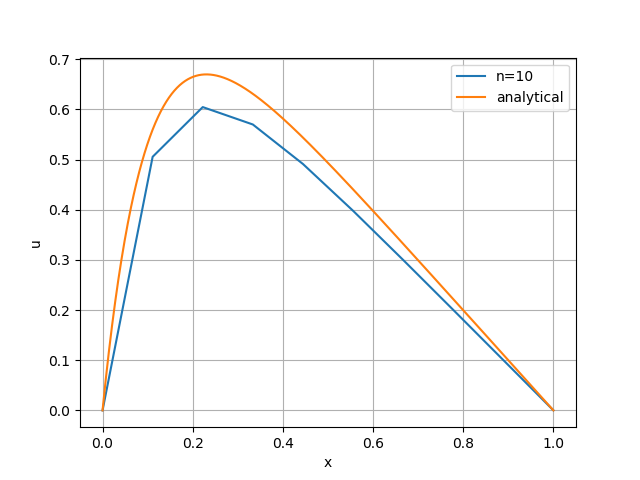
\includegraphics[scale=0.7]{n10.png}
\end{center}
\caption{Exact vs numerical for $n=10$ grid points}
\label{fig:fig1}
\end{figure}

See Figure \ref{fig:fig2}.
\begin{figure}[H]
\begin{center}
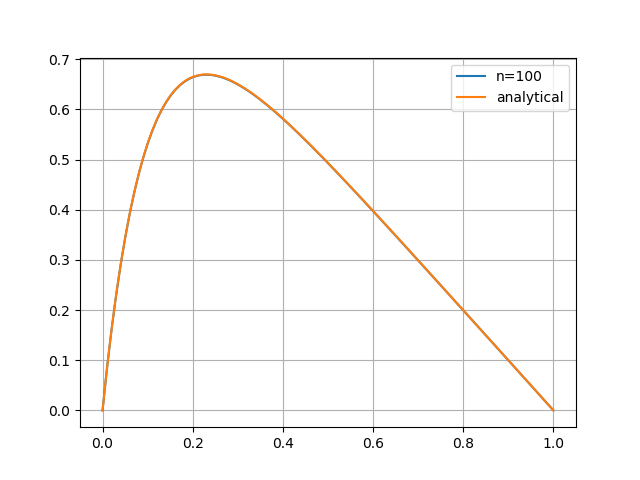
\includegraphics[scale=0.7]{n100.png}
\end{center}
\caption{Exact vs numerical for $n=100$ grid points}
\label{fig:fig2}
\end{figure}

See Figure \ref{fig:fig3}.
\begin{figure}[H]
\begin{center}
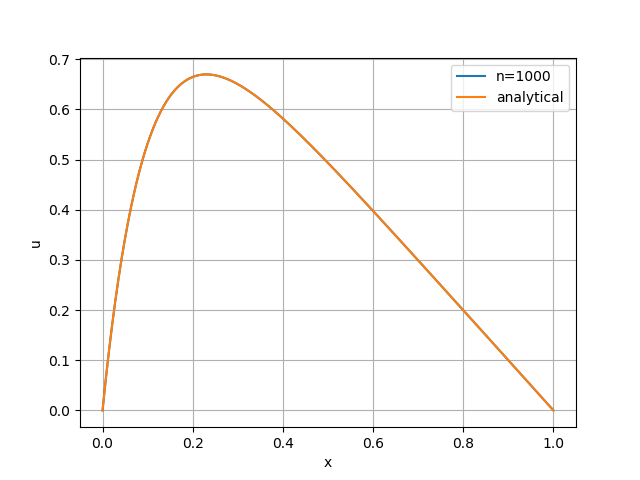
\includegraphics[scale=0.7]{n1000.png}
\end{center}
\caption{Exact vs numerical for $n=1000$ grid points}
\label{fig:fig3}
\end{figure}

(In appendix A, additional figures generated from optimized algo and LU)

Relative error results

See Figure \ref{fig:relerror}.
\begin{figure}[H]
\begin{center}
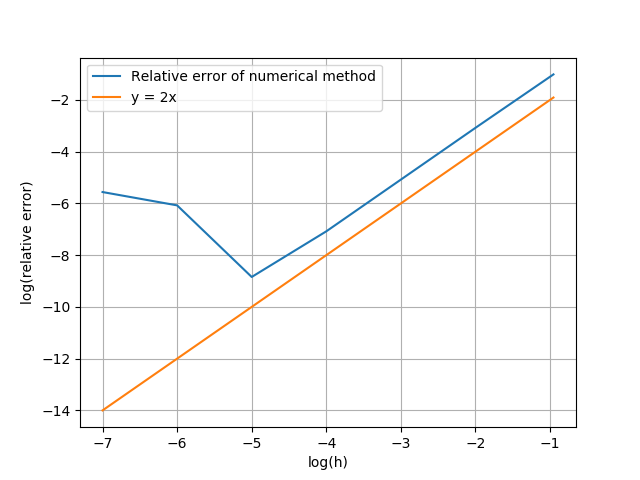
\includegraphics[scale=0.7]{errorestimate.png}
\end{center}
\caption{Relative error of optimized numerical method for $n = 10, 10^2, ...,n=10^7$ grid-points.}
\label{fig:relerror}
\end{figure}

Timing results/efficiency of algorithms

\begin{table}[]
\begin{tabular}{|l|l|l|l|l|l|l|}
\hline
 Method&        $n=10$&  $n=10^2$&  $n=10^3$&  $n=10^4$&  $n=10^5$&  $n=10^6$\\ \hline
 General solver& $1.32 \cdot 10^{-6}$ & $7.94\cdot 10^{-6}$ &  &  &  &  \\ \hline
 Optimized solver& $7.47 \cdot 10^{-7}$ & $1.18$ &  &  &  &  \\ \hline
 LU-decomp& $2.06 \cdot 10^{-4}$&  &  &  &  &  \\ \hline
\end{tabular}
\caption{CPU-time for various methods and grid-points in seconds. The CPU-time is an average of 5 runs on a Intel i7-7700HQ processor}
\label{fig:relerror}
\end{table}

(In appendix A, additional times on different machines, we made test runs on a total of 3 machines. Here we have listed the results from the machine with the best times)

\section{Discussion}
\subsection{Comparing the Exact and Numerical Solution}
From figure \ref{fig:fig1}, \ref{fig:fig2} and \ref{fig:fig3}, we see the obvious trend that the numerical solution converges quickly towards the analytical solution \ref{solution} for increasing $n$. Already for $n=100$ and $n=1000$, the numerical solution is indistinguishable from the analytical as seen in the figures. This trend of fast convergence is expected, since the error caused by the discretization is expected to be proportional to the square of the step-size $h$ according to ....\\

\subsection{Relative Error Estimate}
The relation between the relative error \ref{eq:error} and step-size h is further verified by looking at the log-log plot of the relative error as a function of h \ref{fig:relerror}. For $log(h)$ between $-1$ and $-5$ (corresponding to n between $10$  and $10^5$), the relation is close to linear with slope 2, indicating that the relative error scales as $h^2$ as expected. This relation is however broken for $n>10^5$ due to insufficient machine precision, causing roundoff-errors in the algorithm. This extremal point is close to the estimated...

\subsection{CPU-time for the Different Methods}
For $n = 10^5$ and higher, the solution using LU-decomposition from Armadillo caused the computer to freeze. This is not due to too long CPU-time, but rather too little memory available. Even though we have a sparse matrix, meaning most of the elements are zero, Armadillo need to explicitly store every element in memory with double precision. This results in $10^5 * 10^5 *8B \approx 80$GB, not even including the pointers that also need to be stored in memory. This far exceeds our available 8GB of RAM, making Armadillo's general LU-decomposition unviable for large numbers of grid-points. Our specialized method need only store the diagonal, source function and solution, totaling a mere $3*10^5*8$B$ \approx 2.1$MB

\section{Conclusion}

\newpage
\section*{References}
% Examples:
% [1] Surname, Name. “Title”. Edition. Publisher (Year published)
% [2] Squires, G. L. “Practical Physics”. 4th Edition. Cambridge (2001)

[1] FYS3150/4150 Computational Physics I: Project 1 problem description. Department of Physics, University of Oslo (August 6, 2018)

[2] Jensen, M. H. Lecture


\newpage
\appendix
\renewcommand\thesection{Appendix \Alph{section}:}
\section{Additional Results}

Additional results, e.g. plots generated from optimized algorithm and LU-decomposition, time results on other machines etc.

\end{document}
